\documentclass[hidelinks,12pt]{article}
\usepackage{amsmath}
\usepackage{graphicx}
\usepackage[english]{babel}
\usepackage[utf8]{inputenc}
\usepackage{fancyhdr}
\usepackage{tabularx}
\usepackage{hyperref}
\usepackage{float}
\usepackage{subcaption}
\usepackage{listings}
\usepackage{xcolor}

\definecolor{codegreen}{rgb}{0,0.6,0}
\definecolor{codegray}{rgb}{0.5,0.5,0.5}
\definecolor{codepurple}{rgb}{0.58,0,0.82}
\definecolor{backcolour}{rgb}{0.95,0.95,0.92}

\lstdefinestyle{mystyle}{
    backgroundcolor=\color{backcolour},   
    commentstyle=\color{codegreen},
    keywordstyle=\color{magenta},
    numberstyle=\tiny\color{codegray},
    stringstyle=\color{codepurple},
    basicstyle=\ttfamily\footnotesize,
    breakatwhitespace=false,         
    breaklines=true,                 
    captionpos=b,                    
    keepspaces=true,                 
    numbers=left,                    
    numbersep=5pt,                  
    showspaces=false,                
    showstringspaces=false,
    showtabs=false,                  
    tabsize=2
}

\lstset{style=mystyle}

\hypersetup{
    colorlinks=true,
    linkcolor=cyan,
}

\pagestyle{fancy}
\fancyhf{}
\chead{MIPS Simulator}
\rfoot{\thepage}

\begin{document}

\begin{titlepage}
    \centering
    
\includegraphics[scale=0.5]{../../logo.png}\\[1.0cm]
    \Large INDIAN INSTITUTE OF TECHNOLOGY DELHI\\[1.0 cm]
    \LARGE COL216\\[0.1cm]
    \Large \underline{Report}\\
    \large \[Assignment-3\]
    \LARGE \textbf{MIPS Simulator}


    \rule{\textwidth}{0.2 mm} \\[0.1cm]
    \begin{abstract}
        A simulator is a software that emulates the actions of an entity without actually using the entity.
        Here we attempt to create a cross platform MIPS simulator that emulates all the hardware instructions supported by MIPS.
        This simulator takes as input a MIPS assembly program that translates it into instructions executed by MIPS.
        \\[0.1cm]
    \end{abstract}
    \rule{\textwidth}{0.2 mm} \\[0.1cm]
    \begin{flushright}

        \begin{tabular}{c c}
            \small {Harsh Agrawal}      & \small {2019CS10431} \\
            \small {Saptarshi Dasgupta} & \small {2019CS50447} \\
        \end{tabular}
    \end{flushright}
\end{titlepage}
\tableofcontents
\newpage

\section{Approach}
We implemented a simulator in \verb|C++| for executing MIPS instructions from input assembly code. We divided our program into two modules a \verb|compiler| and a \verb|hardware| module.
These modules perform different functions as outlined below
\subsection{Compiler}
\begin{itemize}
    \item This module takes as input the assembly program and parses the tokens according to the syntax specifications of MIPS assembly programs.
    \item This module assembles the program into a sequence of instructions that can be executed according to the hardware specifications.
    \item It also generates appropriate syntax errors if an erreneous expression or an unidentified token is encountered.
    \item The compiler checks the encodibility of instructions into 4 bytes (without actually encoding it) using the size of operands involved.
\end{itemize}
\subsection{Hardware}
\begin{itemize}
    \item This module emulates a subset of instructions provided by MIPS. They are \verb|add, mul, sub, slt, addi, bne, beq, j, lw, sw|.
    \item The module maintains a record of all the register and memory values and modifies them according to the instruction specifications.
    \item It generates appropriate exceptions on performing prohibited actions like out of bounds memory access and reserved register access.
\end{itemize}

\section{Testing}
We employed both automated and manual modes of testing. The automated mode helped establish the correctness of the arithmetic operations like \verb|add, sub, mul, slt, addi| while the manual mode helped us evaluate the correctness for \verb|lw, sw, bne, beq, j| instructions.
\subsection{Automated}
We wrote a \verb|python3| script that generates random MIPS assembly statements for the arithmetic instructions \verb|add, mul, sub, slt, addi|.
The script executes these instructions using our program and stores the register values after each step. The same program is then fed into the \verb|spim| simulator and
the register values are queried and stored. The two sets of register values are checked against each other for each \verb|ASM| statement in the test case.
All communication with the executed process occurs through unix pipes and a \verb|PTY| interface.
To install the dependencies, enter the following commands. \\[0.1cm]
\begin{lstlisting}[language=bash]
    $ sudo apt install spim
    $ python3 -m pip install -r requirements.txt
    $ python3 tester.py -n 20 -m 30 
\end{lstlisting}
The last command will run $20$ test cases with $30$ instructions in each test case and print a test log with the result of each test case.
The generated test cases are saved in a the \verb|./output| directory by default but can be changed by supplying the \verb|-o, --output| command line flag to the python script\\

\textbf{Note:} The test cases generated by this method is saved in the \verb|./tests/automated| directory for reference

\subsection{Manual}
We have also included some manual \verb|ASM| files in the \verb|./tests/manual| directory. These test cases are meant to test the correctness of \verb|lw, sw, beq, bne, j| instructions.
These tests are present in the \verb|./tests/manual/| folder.
\begin{itemize}
    \item \verb|arithmetic:| This test case checks the correctness of \verb|add, mul, sub|. We have also handled overflows and raised an arithmetic overflow exception in such a case.
    \item \verb|conditional:| \verb|if-then-else| implemented using \verb|bne, beq ,j|. These cases test the branching conditions in an assemblt program and ensure that the execution jumps to a logically correct statement.
    \item \verb|looping:| Implementing loops for counter and fibonacci numbers. We have implemented loops using jump statements and matched the output with the expected output. The fibonacci numbers and a simple counter are the most intuitive examples.
    \item \verb|stacks:| We implemented stacks using the \verb|lw| and \verb|sw| instructions. The push and pop methods were implemented and the expected values were checked.
    \item \verb|errors:| Extensive testing for errors with invalid register, labels, integers, out of bounds memory addressing,
          non-word aligned adresses and accessing kernel reserved registers
\end{itemize}

\subsection{Results}
We evaluated the results of these tests in both the automated process and the manual process. Based on our testing we conclude the following:
\subsubsection{Automated}
The register contents of \verb|spim| and our simulator were compared and all the test cases passed as expected. The snapshots of the results are attached below.\\

Since our approach allows us to test for arbitrarily large test cases we were able to extensively test our implementation. The results showed that our implementation is robust as it passed all sorts of test cases.\\

We could not match our output with \verb|spim| output in cases where integer overflow occured. This is because spim automatically handles arithmetic overflows whereas our program raises an arithmetic overflow exception.
Since our simulator aims to emulate the hardware as closely as possible we decided to not handle the exception by default.
\begin{figure}[H]
    \centering
    \begin{subfigure}[t]{\textwidth}
        \centering
        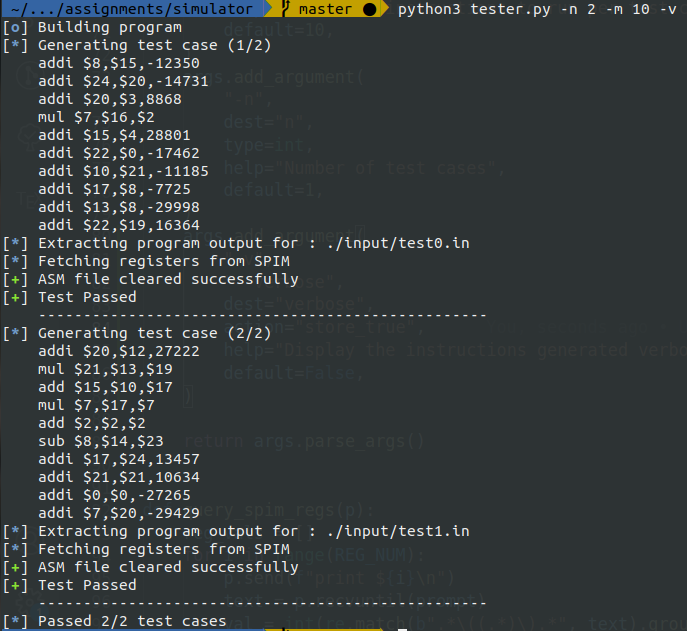
\includegraphics[scale=0.4]{n2_m10.png}
        \caption{2 test cases each with 10 instructions}
    \end{subfigure}
    \begin{subfigure}[t]{\textwidth}
        \centering
        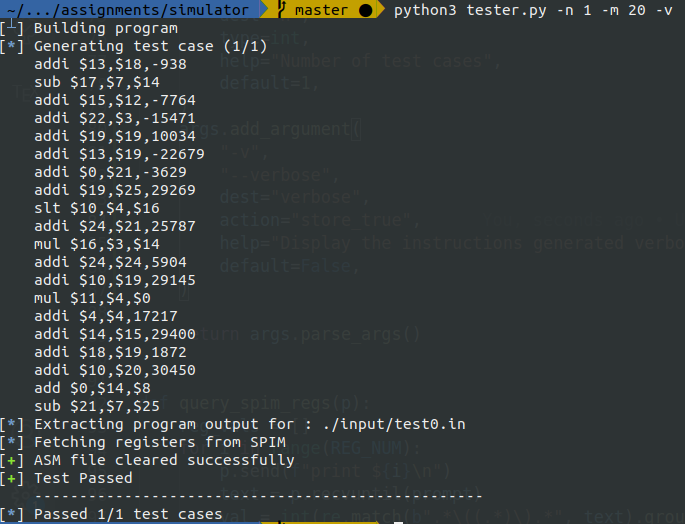
\includegraphics[scale=0.4]{n1_m20.png}
        \caption{1 test case with 20 instructions}
    \end{subfigure}
    \caption{Automatic evaluation}
\end{figure}

\subsubsection{Manual}
We tested for all the test cases described above.
Some of the outputs are shown below
\begin{figure}[H]
    \centering
    \begin{subfigure}[t]{\textwidth}
        \centering
        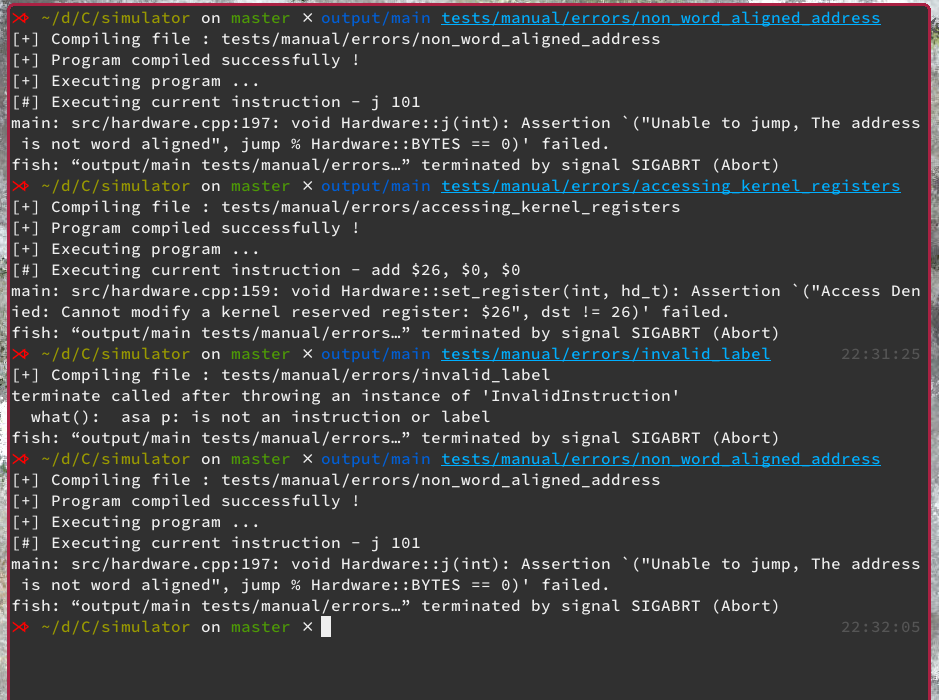
\includegraphics[scale=0.4]{manual_errors.png}
        \caption{test cases causing different errors}
    \end{subfigure}
    \begin{subfigure}[t]{\textwidth}
        \centering
        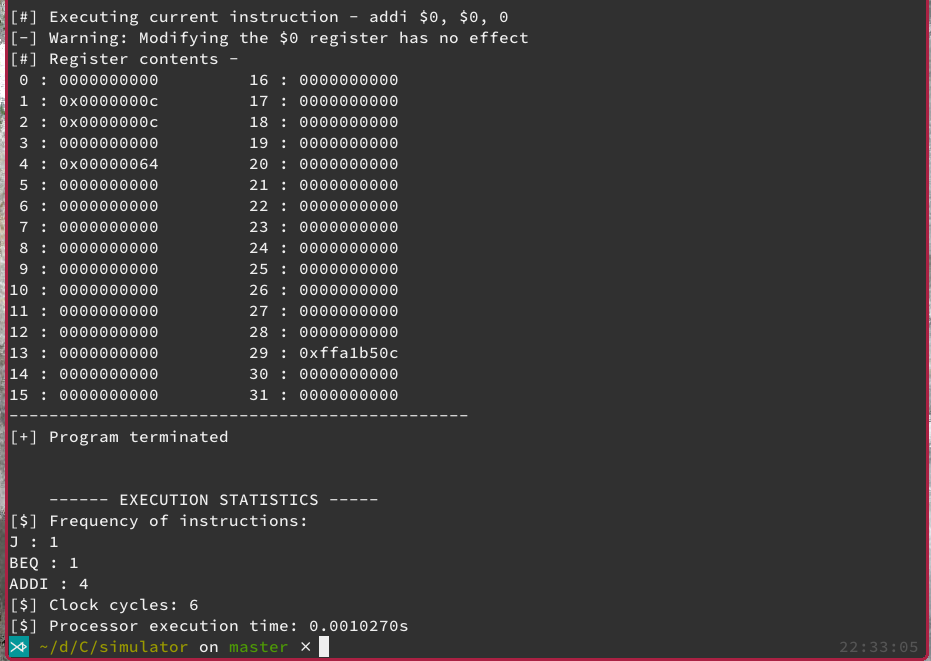
\includegraphics[scale=0.4]{manual_conditional.png}
        \caption{1 test case with if-then-else implemented using beq}
    \end{subfigure}
    \caption{Manual evaluation}
\end{figure}


\section{Assumptions}
\begin{itemize}
    \item We have assumed that the maximum memory available to any user program is $2^{20}$ bytes. This includes the memory required for storing instructions and the stack memory.
    \item We have assumed 32 registers for MIPS each of them storing 32 bits. We have hardwired the register \verb|$0| to the value $0$ as is the case in MIPS hardware. We have also restricted use of kernel reserved registers \verb|$26, $27|.
    \item We have assumed that exactly 1 clock cycle is required for each of the instruction to display the execution statistics.
    \item We have enforced tight syntax rules to enforce good coding practice. We disallow certain instructions like (a) \verb|lw $5, ($29)| and (b) \verb|lw $5, 40231|.
          The first instruction skips supplying the offset to the register and the second one involves raw memory access. We have used actual memory addresses allocated by the OS to initialize the stack pointer as will be the case for any program running on an actual harware.
          This makes our implementation more scalable and robust as compared to using indexes from $0 - 2^{20}$ to reference memory which will most likely be a reserved address and lead to segmentation fault.
    \item Our implementation also enforces using numeric registers instead of their named counterparts. For example \verb|$5| is allowed but its named counterpart \verb|$a1| is disallowed
    \item We have enforced the use of a whitespace between the operand and its arguments. For example \verb|add$4,$5,$6| is disallowed as there is no whitespace between \verb|add| and \verb|$4|
    \item We have implemented branching instructions like \verb|beq, bne, j| to take only labels and instruction numbers as the last argument.
\end{itemize}

\end{document}

